\section{Results}
\label{Results}
\subsection{\psitwos-to-\jpsi ratio as function of multiplicity}
With the signal yields determined from the fitting to dimuon invariant mass distributions, the efficiency ratios estimated from simulation and calibrated control samples, and the systematic uncertainties, the ratio of \psitwos and \jpsi production cross-sections are measured as a function of different multiplicity variables. As mentioned in Sec~\ref{Efficiency determination}, the multiplicity distribution of \jpsi and \psitwos can be treated as the same, and due to the large uncertainty of \psitwos multiplicity distribution, the x-coordinate representing the multiplicity is directly the mean value of \jpsi multiplicity distribution in each bin, normalized by the mean value of multiplicity of NoBias data. The box represents systematic uncertainty and the error bar represents the statistical uncertainty. In this analysis statistical uncertainty dominates.
The normalized \psitwos-to-\jpsi ratio as function of $N_{\rm tracks}^{\rm PV}$ in $p$Pb and Pb$p$ collisions is shown in Figure~\ref{NormPVN}.
\begin{figure}[H]
\begin{center}
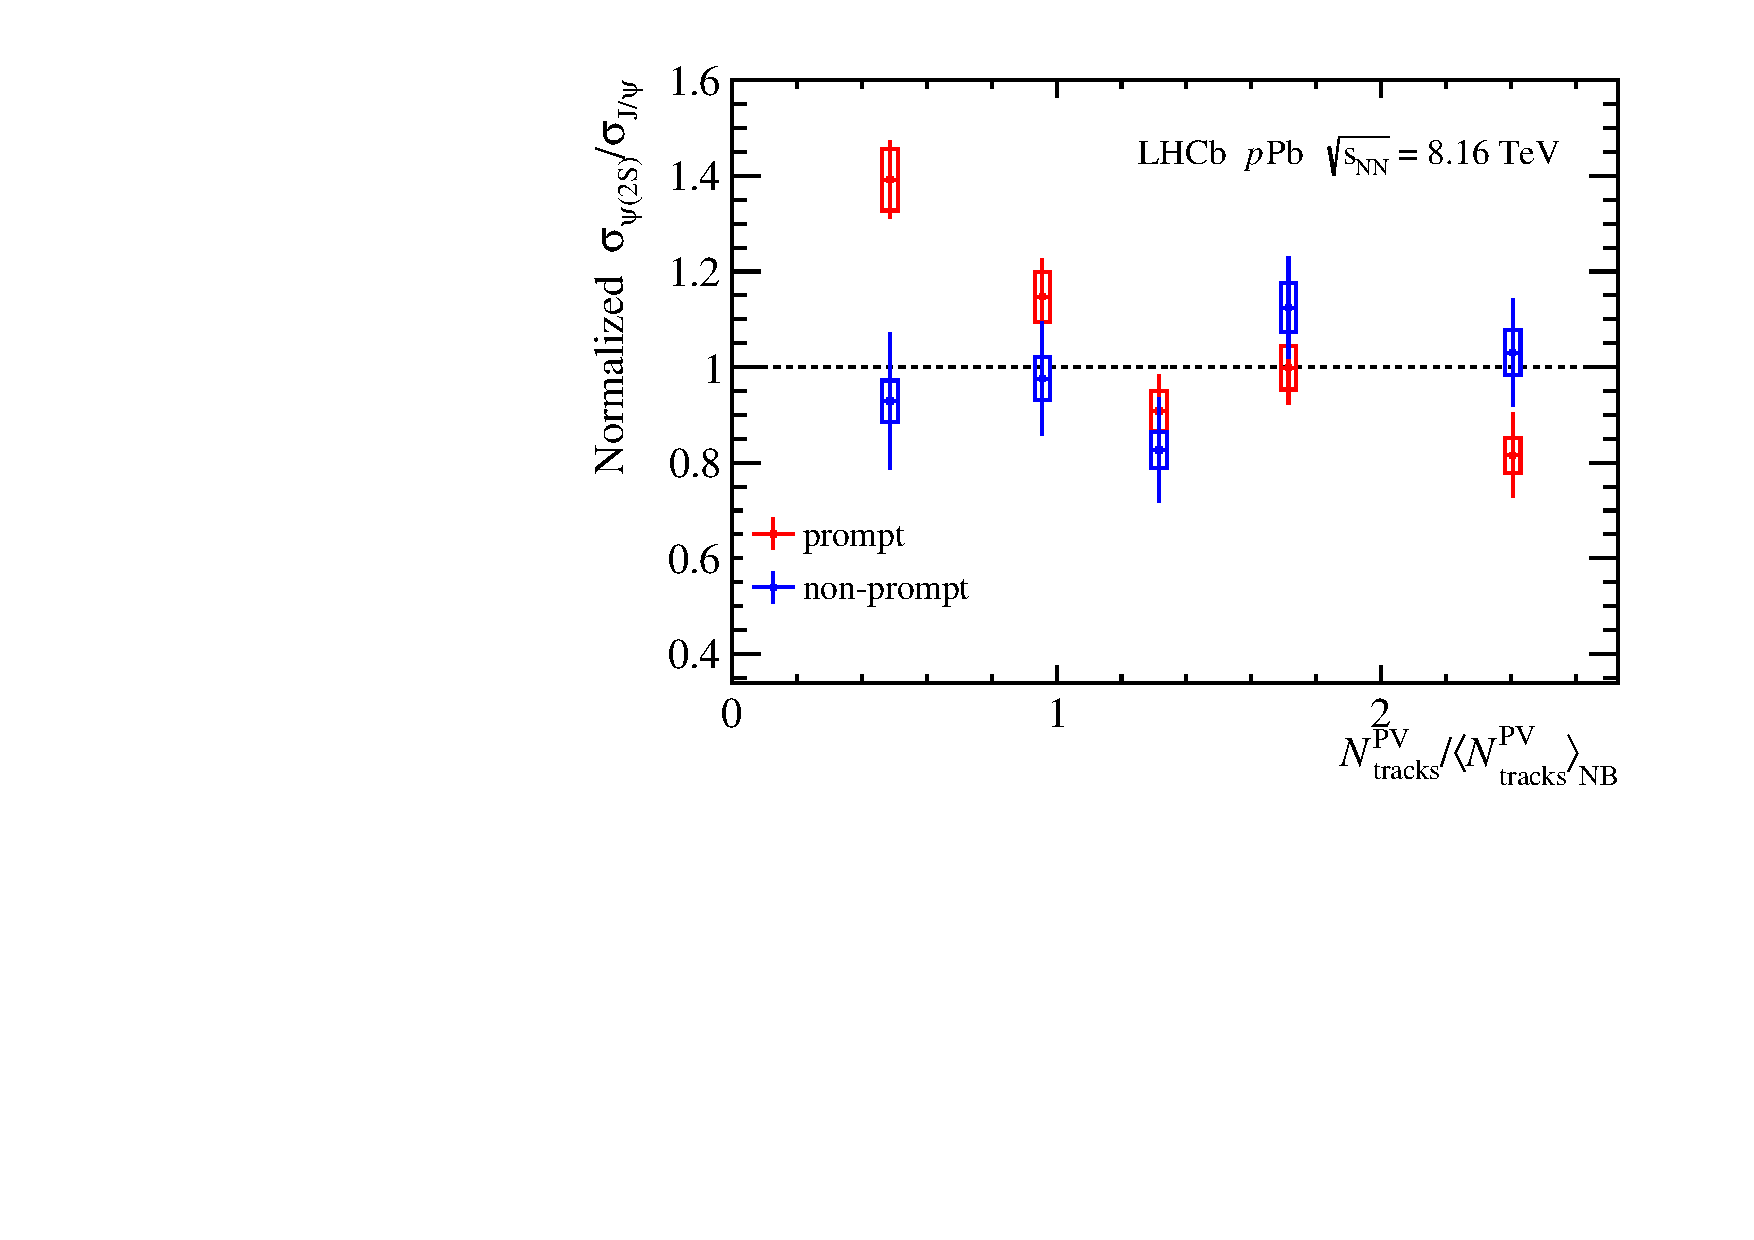
\includegraphics[width=0.49\linewidth]{pdf/pPb/Workdir/Result/All.pdf}
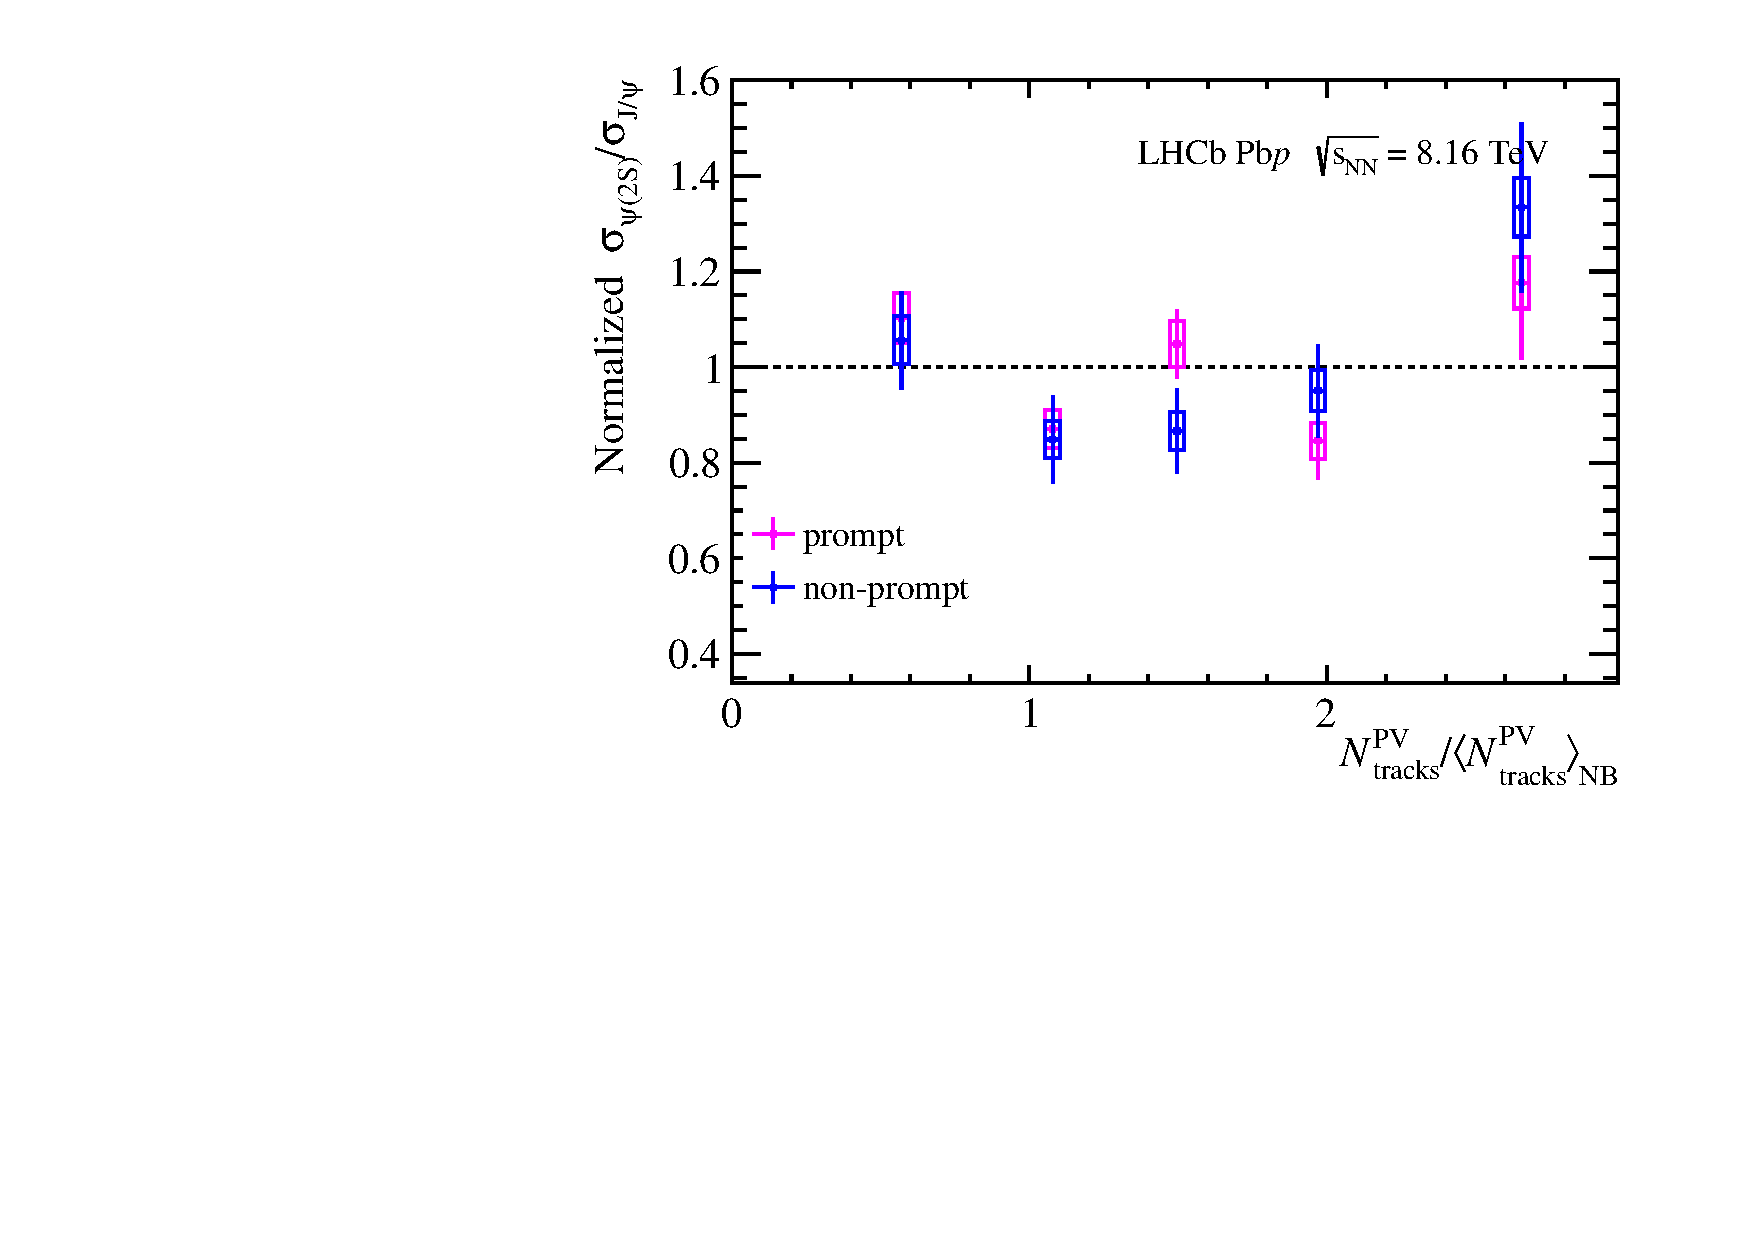
\includegraphics[width=0.49\linewidth]{pdf/Pbp/Workdir/Result/All.pdf}
\end{center}
\caption{Normalized \psitwos-to-\jpsi ratio as function of normalized $N_{\rm tracks}^{\rm PV}$ in $p$Pb (left) Pb$p$ (right).}
\label{NormPVN}
\end{figure}
We can conclude that in $p$Pb collisions the prompt ratio decrease with increasing $N_{\rm tracks}^{\rm PV}$, while in Pb$p$ collisions, we can not conlude any significant trend with $N_{\rm tracks}^{\rm PV}$. For \jpsi and \psitwos from $b$ we do not find any dependence between the ratio and multiplicity.
If we compare the prompt ratio (not normalized), we should include the uncertainties branching fraction and the comparison is in Figure~\ref{ComparePVN}.
\begin{figure}[H]
\begin{center}
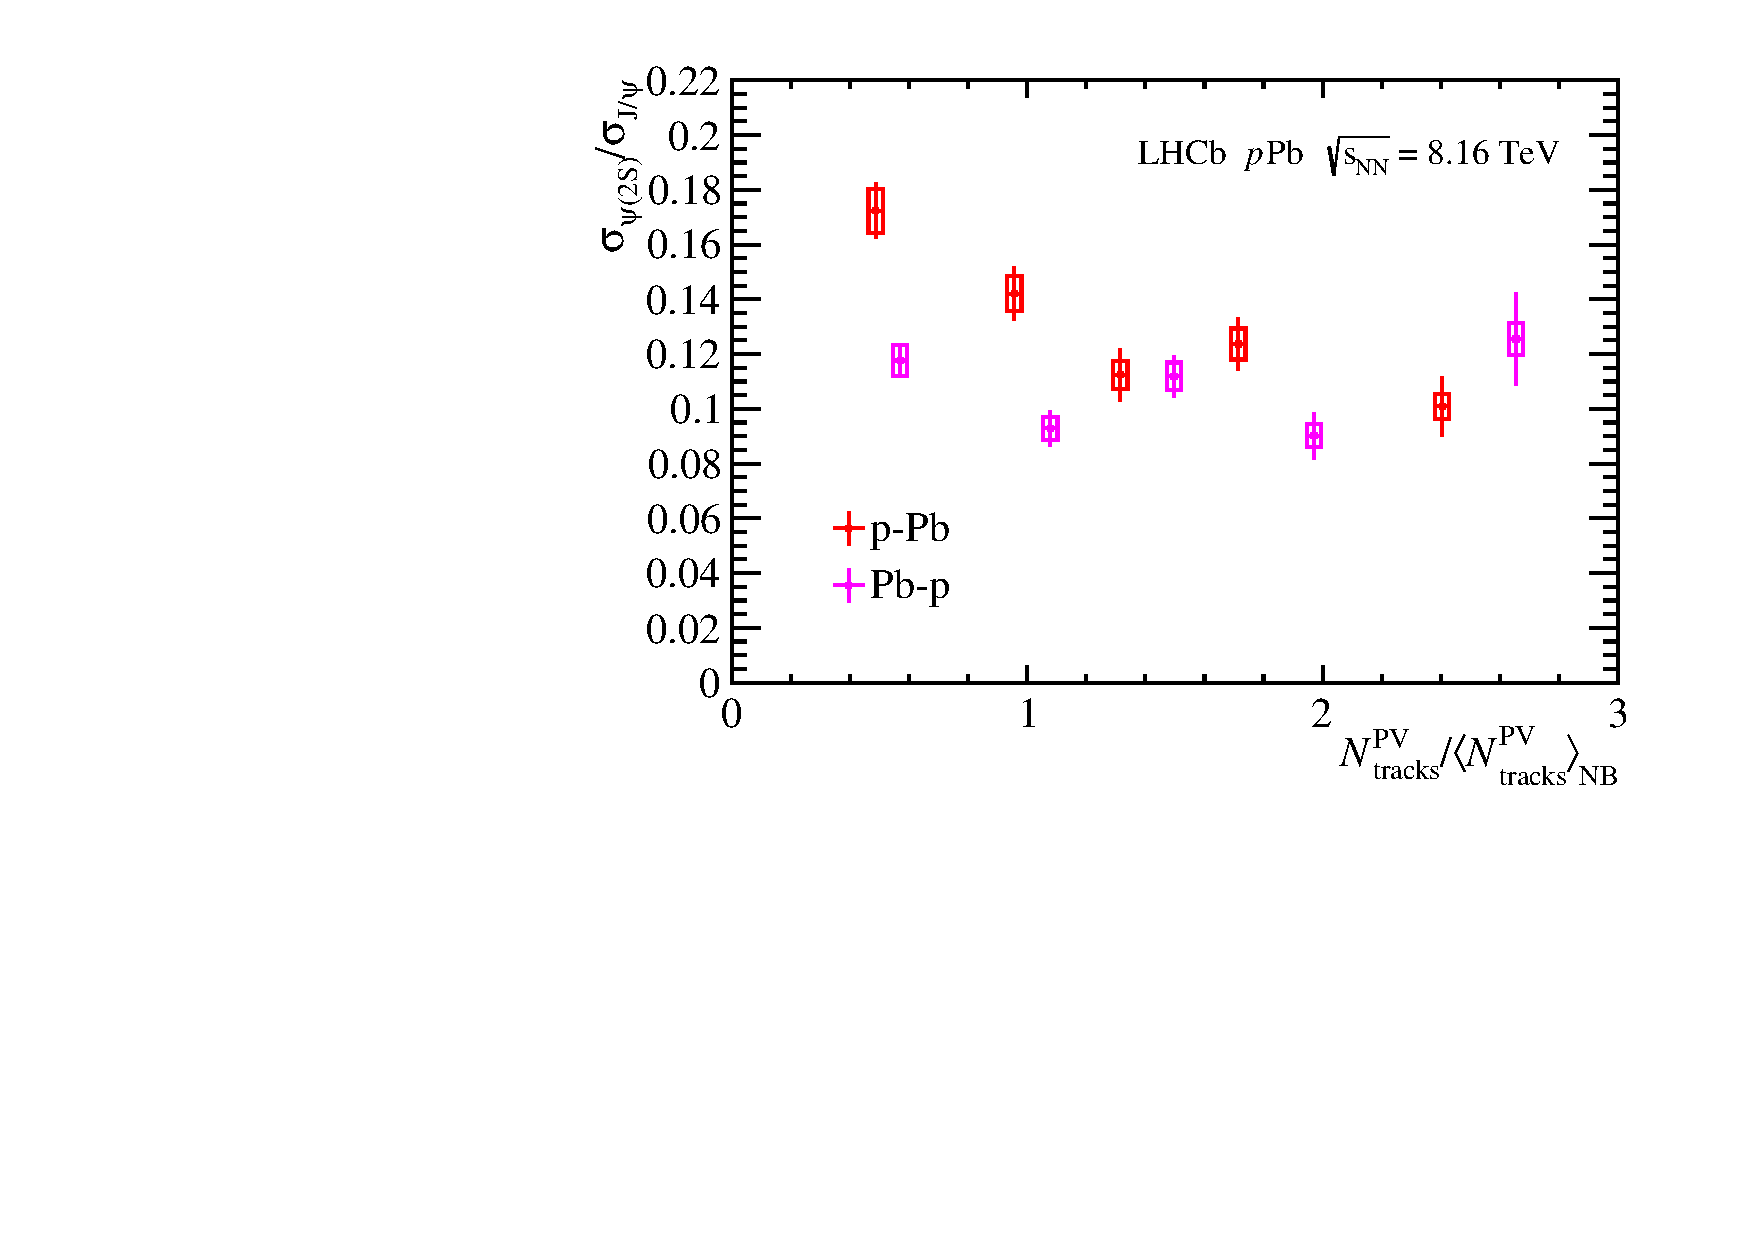
\includegraphics[width=0.7\linewidth]{pdf/pPb/Workdir/Result/Norm.pdf}
\end{center}
\caption{\psitwos-to-\jpsi ratio as function of normalized $N_{\rm tracks}^{\rm PV}$.}
\label{ComparePVN}
\end{figure}
We find the ratio in Pb$p$ is generally lower than that in $p$Pb collisions. This could results from the higher charged particle multiplicity in Pb$p$ collisions, where \psitwos, with lower bounding energy, is easier to dissociate when interacting with higher amount of co-moving particles. But if this is valid, we should also observe a decreasing trend of the ratio with increasing multiplicity, which is indeed not.
We furtherly measure the normalized ratio and ratio as functions of $N_{\rm fwd}^{\rm PV}$, as shown in Figure~\ref{NormFor}. It comes to an agreement with the results when measuring by $N_{\rm tracks}^{\rm PV}$. The ratio of non-prompt signals is roughly constant with multiplicity in $p$Pb and Pb$p$ collisions. And ratio of prompt signals decreases with increasing $N_{\rm fwd}^{\rm PV}$ in $p$Pb, but not in Pb$p$ collisions. 
If we compare the ratio in $p$Pb and Pb$p$ collisions, the ratios in Pb$p$ collisions are generally lower than that in p$Pb$ collisions. But still, we do not observe a decreasing trend like in $p$Pb collisions. Some extra mechanisms might be needed to explain the phenomenon. Since for both $N_{\rm tracks}^{\rm PV}$ and $N_{\rm fwd}^{\rm PV}$ as multiplicity variables, we get the similar outcomes.
\begin{figure}[H]
\begin{center}
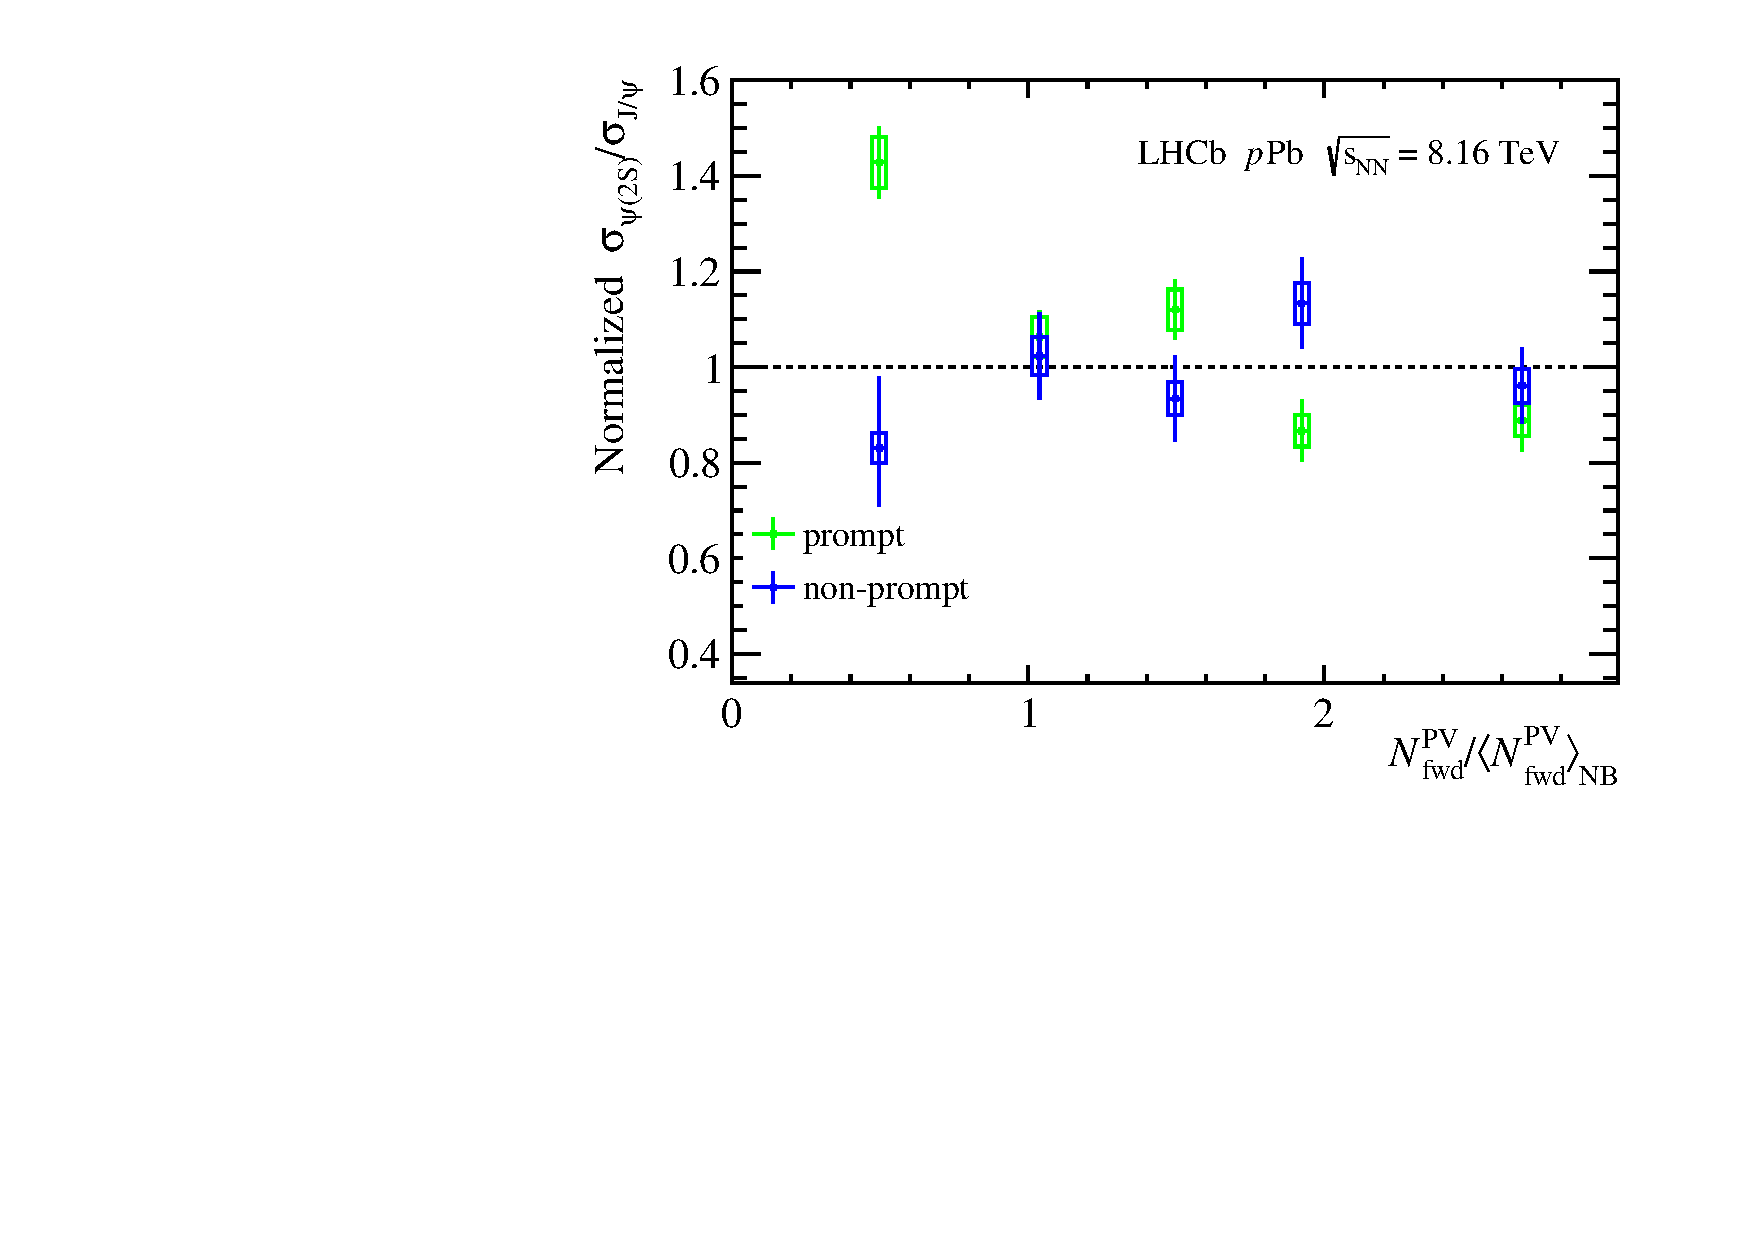
\includegraphics[width=0.49\linewidth]{pdf/pPb/FWorkdir/Result/All.pdf}
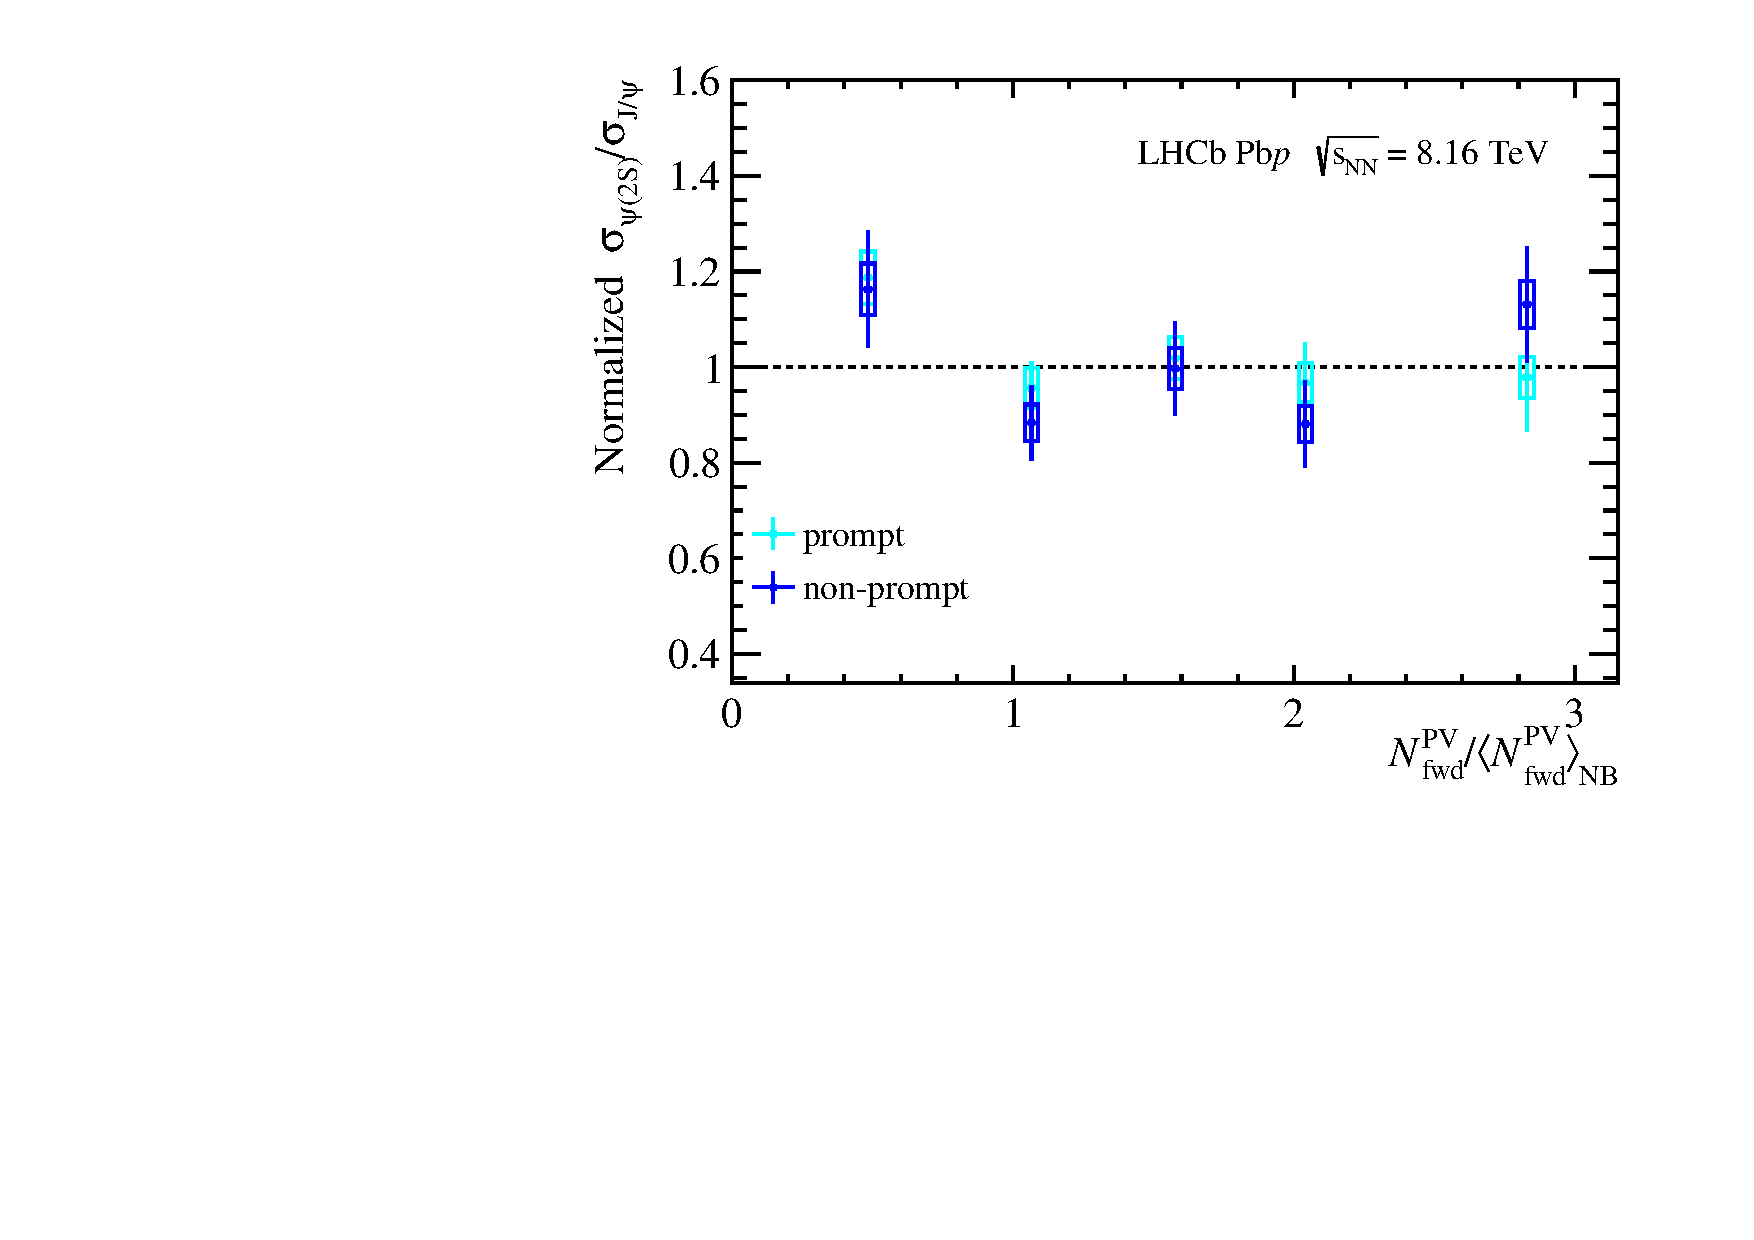
\includegraphics[width=0.49\linewidth]{pdf/Pbp/FWorkdir/Result/All.pdf}
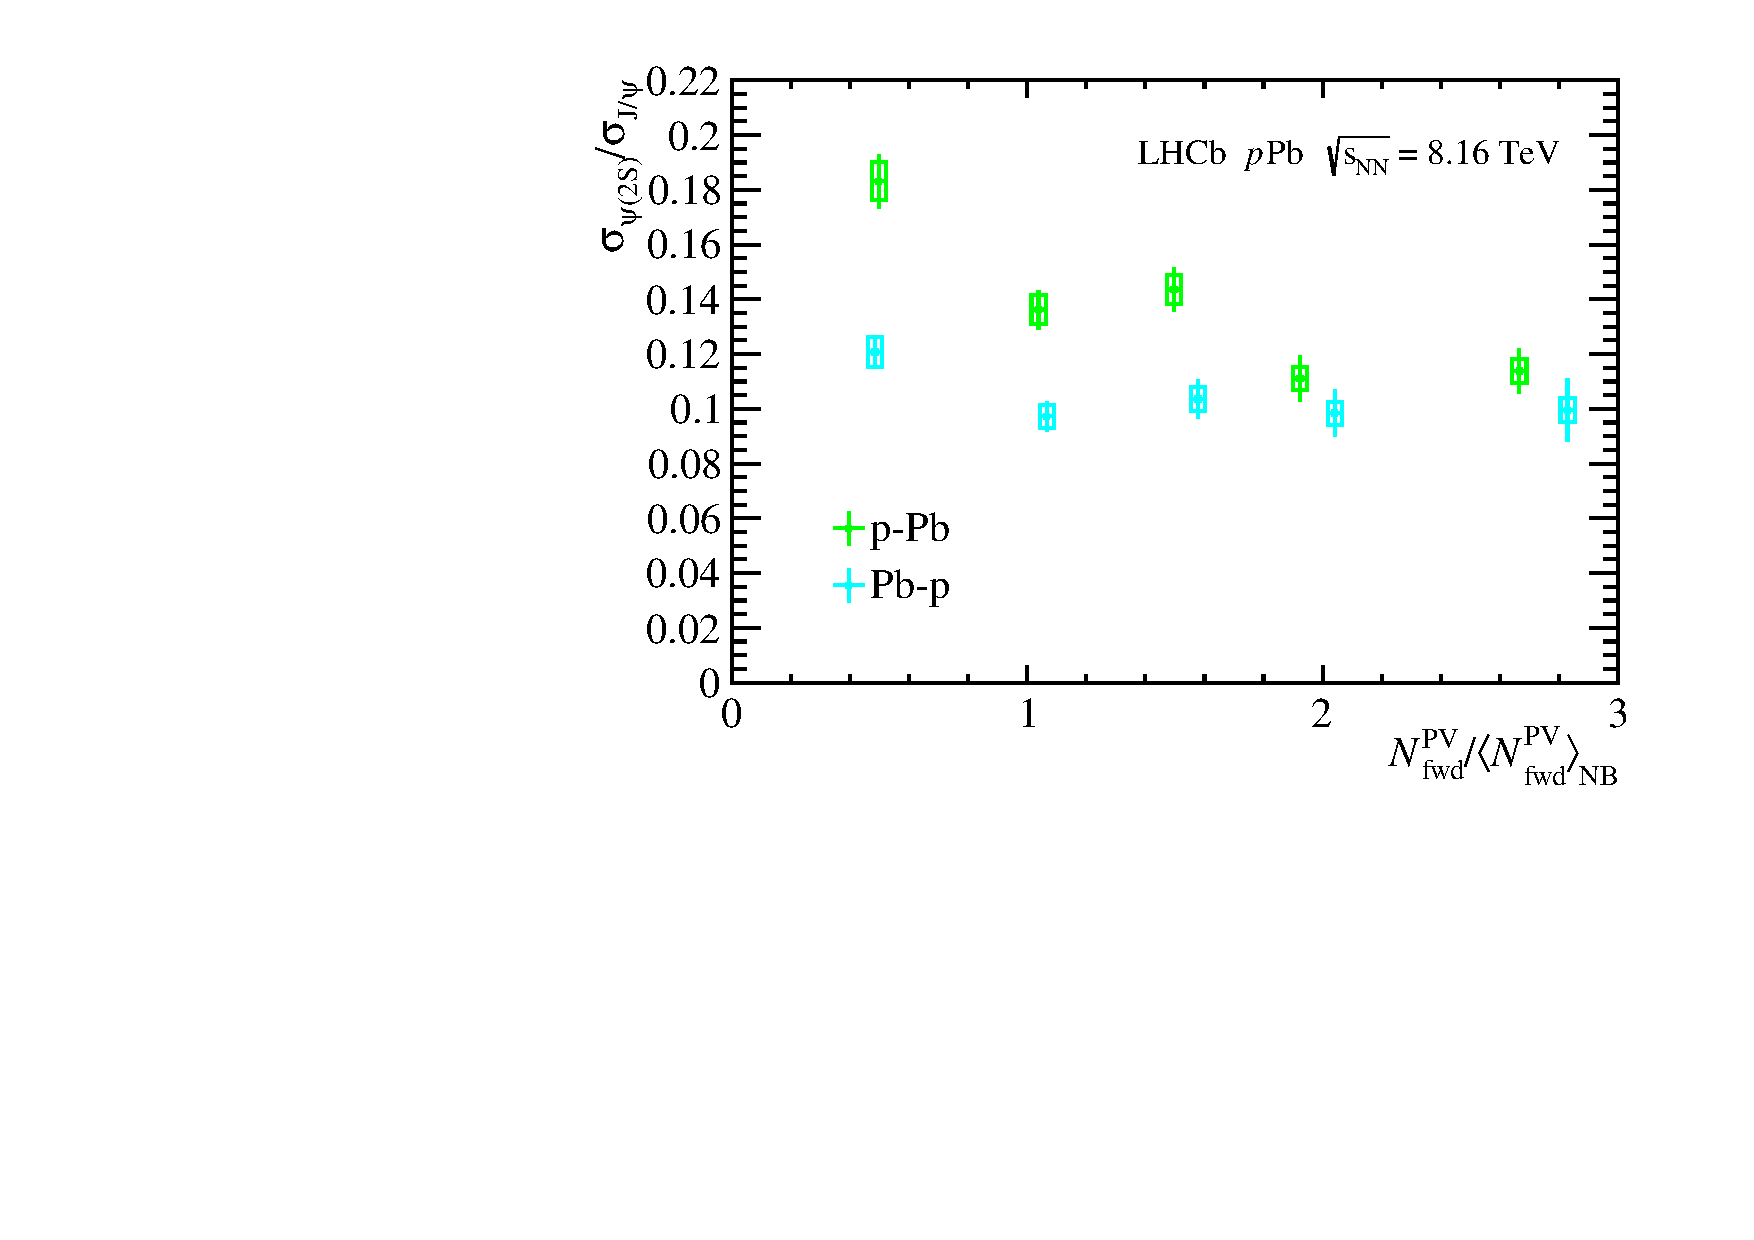
\includegraphics[width=0.7\linewidth]{pdf/pPb/FWorkdir/Result/Norm.pdf}
\end{center}
\caption{Normalized \psitwos-to-\jpsi ratio as function of normalized $N_{\rm fwd}^{\rm PV}$ in $p$Pb (left) Pb$p$ (right).}
\label{NormFor}
\end{figure}
When multiplicity is measured by $N_{\rm bwd}^{\rm PV}$, as shown in Figure~\ref{NormBack}, for ratio of prompt signals, the decreasing trend is much slower with increasing $N_{\rm bwd}^{\rm PV}$ in $p$Pb collisions, and for Pb$p$, the ratio for both prompt and non-prompt signals are roughly constant. Since $N_{\rm bwd}^{\rm PV}$ are measured in backward direction, the rapidity range is non-overlapping with where we measure the charmonia production, and co-mover effect is thought to not exist. Additionally, if QGP is not produced, the ratio should keep constant with $N_{\rm bwd}^{\rm PV}$. The subtle decreasing trend for ratio of prompt signals could result from the correlation between $N_{\rm bwd}^{\rm PV}$ in $p$Pb collisions. Similarly, there is an overall reduction on the ratio in Pb$p$ collisions since the mean value of charged particle multiplicity is higher, which results in an overall larger amount of co-moving particles. But still, in Pb$p$ collisions, no dependence was found between ratio and $N_{\rm bwd}^{\rm PV}$.
\begin{figure}[H]
\begin{center}
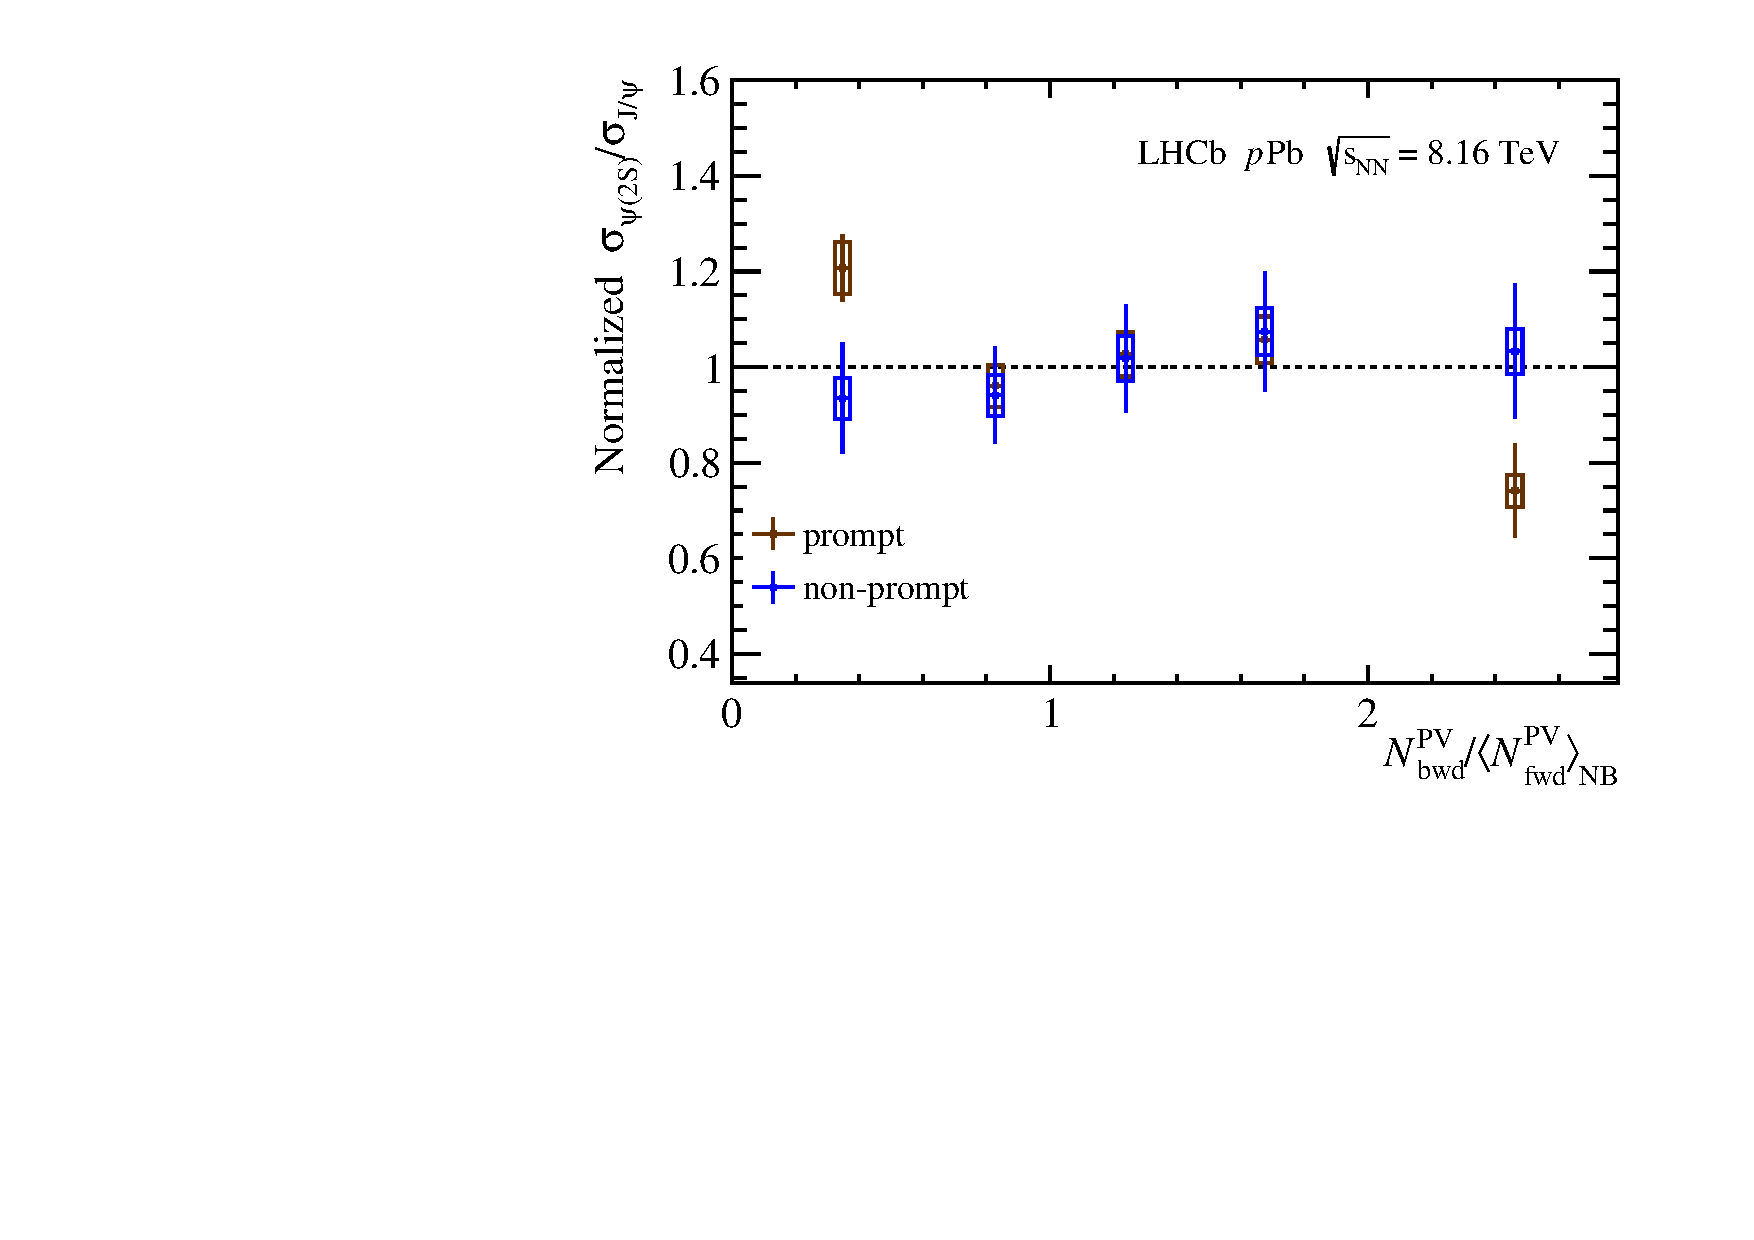
\includegraphics[width=0.49\linewidth]{pdf/pPb/BWorkdir/Result/All.pdf}
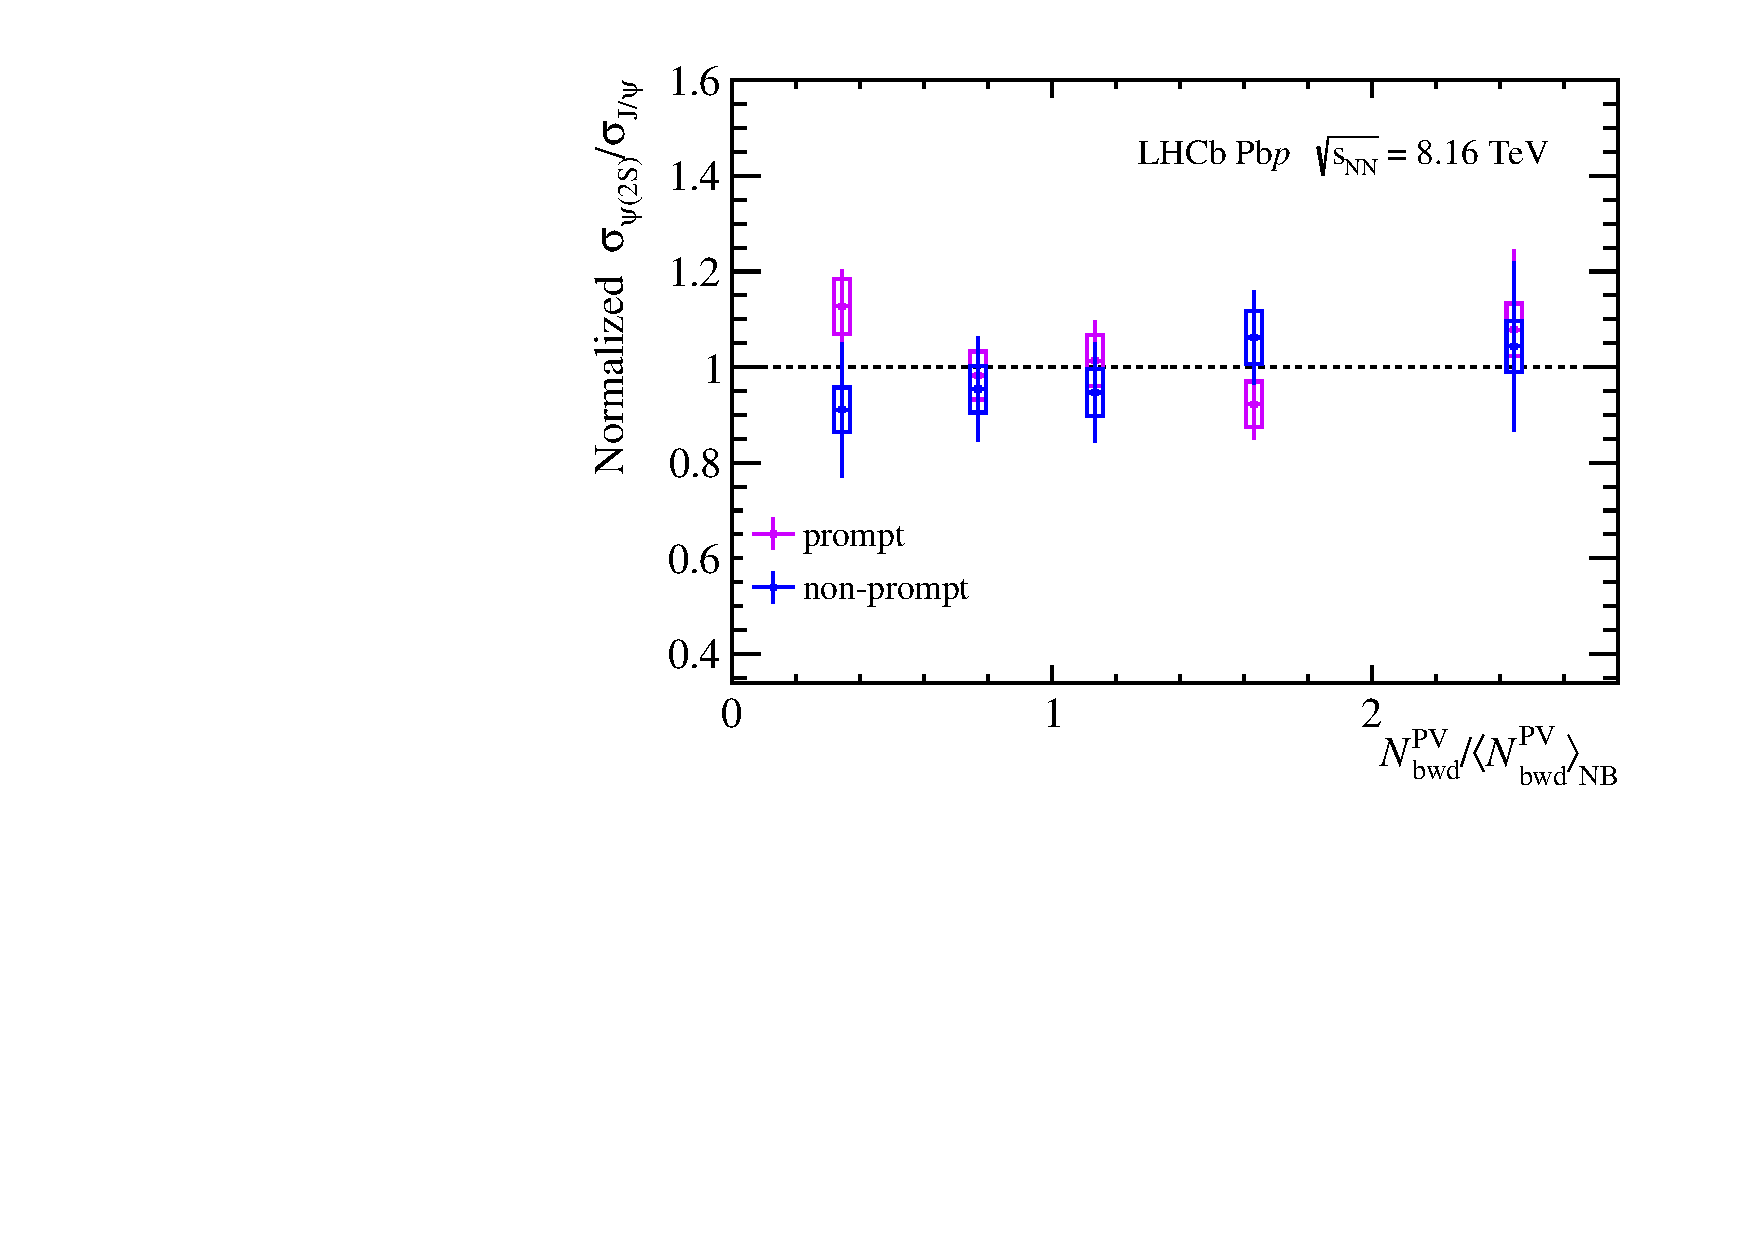
\includegraphics[width=0.49\linewidth]{pdf/Pbp/BWorkdir/Result/All.pdf}
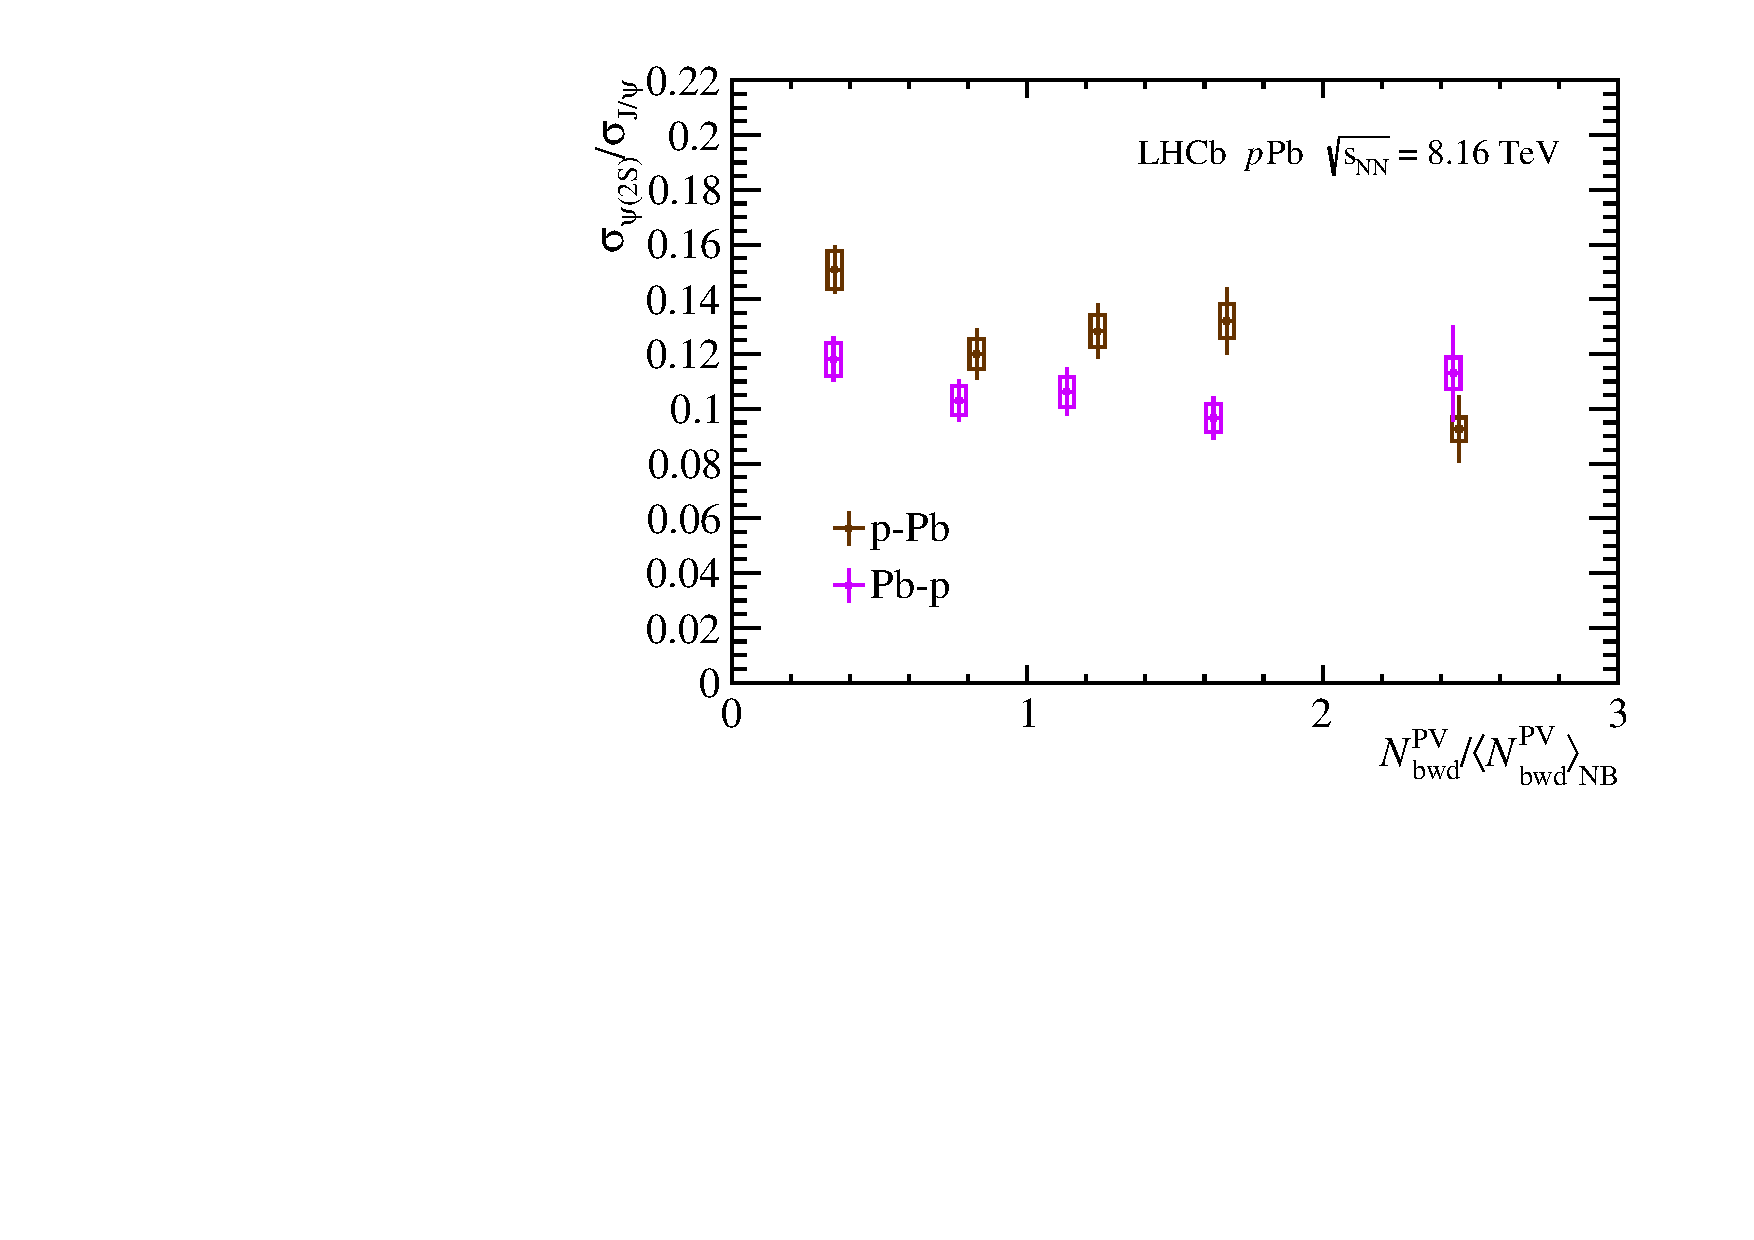
\includegraphics[width=0.7\linewidth]{pdf/pPb/BWorkdir/Result/Norm.pdf}
\end{center}
\caption{Normalized \psitwos-to-\jpsi ratio as function of normalized $N_{\rm fwd}^{\rm PV}$ in $p$Pb (left) Pb$p$ (right).}
\label{NormBack}
\end{figure}

\subsection{Comparison in different collision systems}
The multiplicity dependence of \psitwos to \jpsi ratio in different collision systems is compared as shown in Fig~\ref{pppPb}. 
\begin{figure}[H]
  \begin{center}
  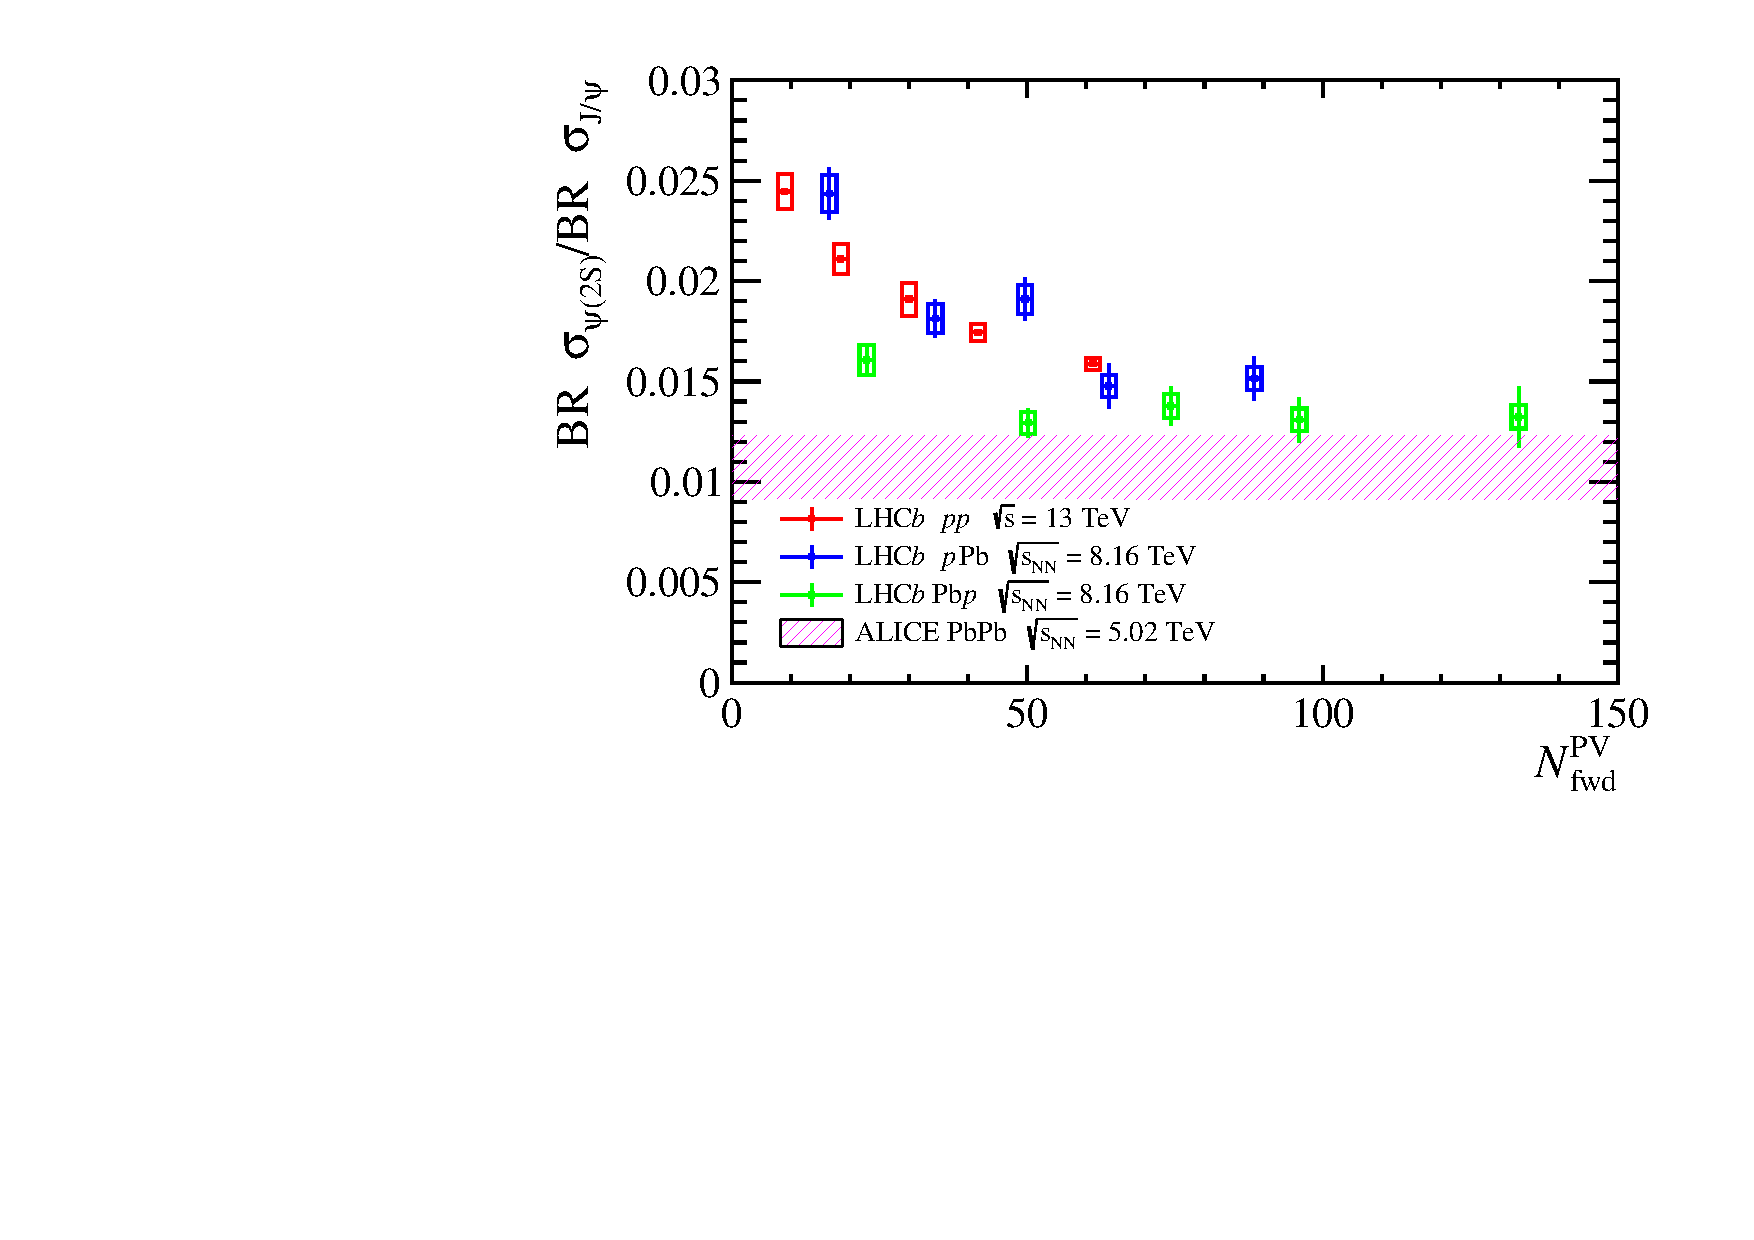
\includegraphics[width=0.7\linewidth]{LHCb-latex-template/latest/latex/pdf/pPb/FWorkdir/Result/pppPb.pdf}
  \end{center}
  \caption{Comparisons on the ratio of \psitwos/\jpsi in $pp$, $p$Pb (Pb$p$) and PbPb collisions~\cite{ALICE:2022jeh}.}
\label{pppPb}
\end{figure}
The multiplicity dependence in $p$Pb collisions is consistent with that in $pp$ result, suggest a similar environment in the final stages in both collision systems. It is within expectation since both are measured in the $p$ going direction, suggesting a similar environment. However, in Pb$p$ collisions, where the charmonia and multiplicity are measured in the $Pb$-going direction, a higher baryon density will achieve, resulting in an environment closer to PbPb collisions. Therefore, a slower decreasing trend is observed in Pb$p$ collisions, which is very close to the result in PbPb collisions measured by ALICE~\cite{ALICE:2022jeh}. A transition phenomenon from small collision systems to large systems is observed.





